\begin{abstract}
A model can learn to answer a problem more reliably while losing alternative
correct solutions. Reinforcement learning with verifiable rewards (RLVR)
provides little feedback about this loss: a repeated success and a different
success receive the same reward. We introduce \mb{}, five executable domains
that identify distinct verified outputs for the same prompt, and ReplayMaxRL,
which combines learning from fresh samples with memory of verified successes.
The same execution keys serve both measurement and replay: each retained key
receives equal weight, even when it becomes rare in fresh rollouts. Across
three model scales, adding replay to Dr.GRPO improves held-out correctness and
sampled verified support. Replay also complements MaxRL at both scales with
complete comparisons; the available 3B results and harder-level comparisons
show where this evidence remains incomplete. An idealized analysis explains
why binary rewards can amplify common modes and how replay can counter that
pressure. The results distinguish learning to succeed from preserving verified alternatives.
\end{abstract}

\begin{figure}[H]
  \centering
  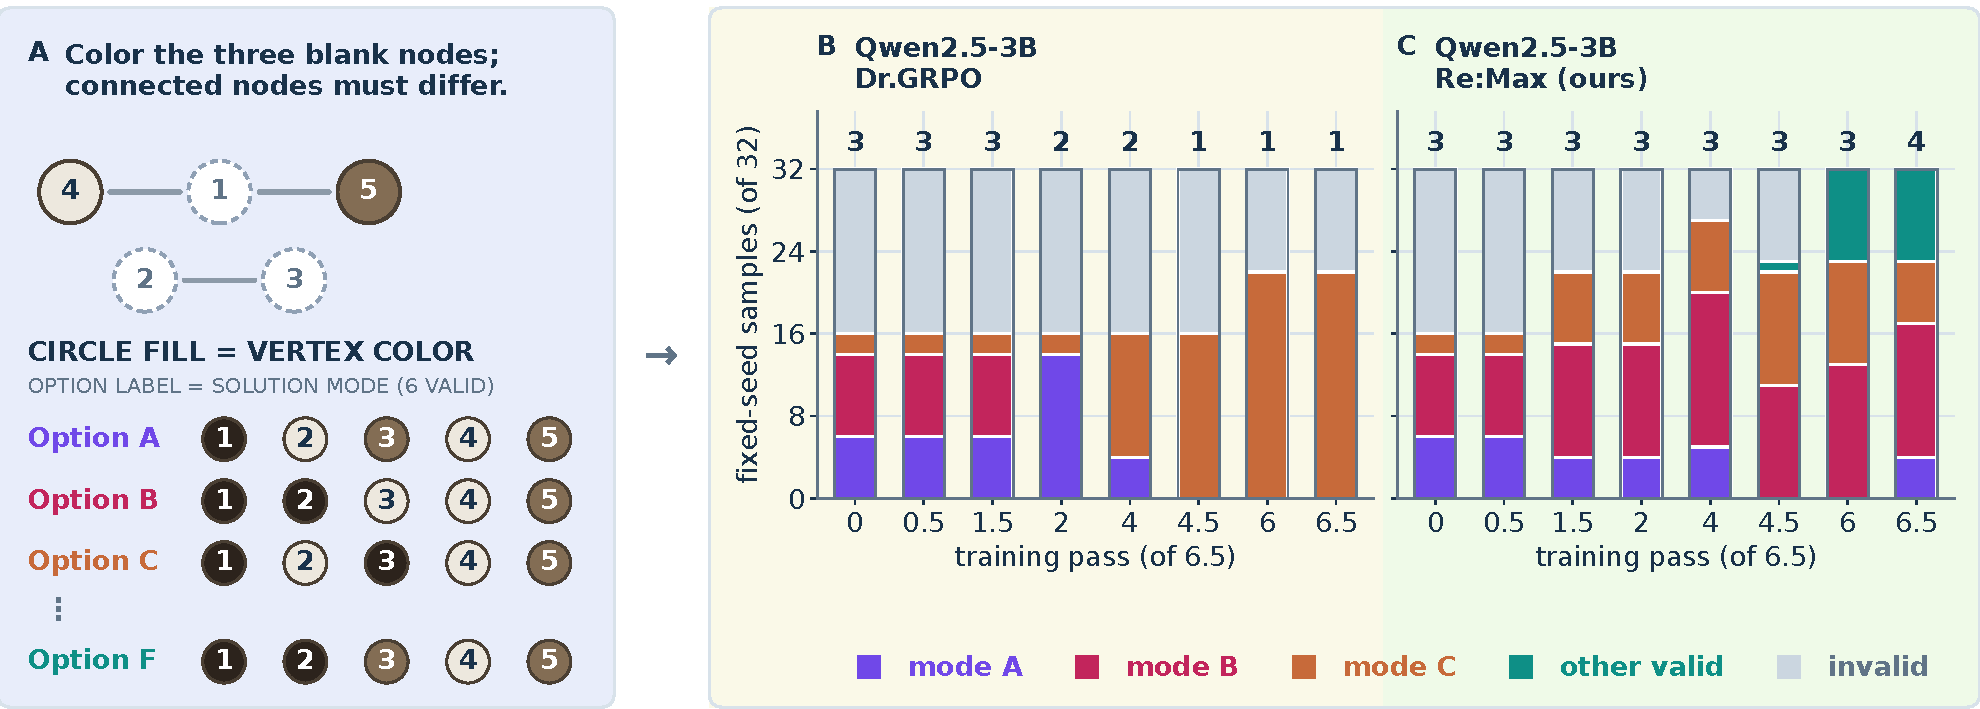
\includegraphics[width=\linewidth]{figures/modecollapse_story.pdf}
  \caption{\textbf{Correctness can rise while sampled alternatives narrow.}
  One graph admits six valid colorings. Bars pool four eight-sample draws from
  matched Qwen2.5-3B runs. At pass 6.5, Dr.GRPO produces 22/32 correct outputs
  from one mode; ReplayMaxRL produces 32/32 across four. Circle fills mark
  vertex colors; dashed rings mark vertices left uncolored in the prompt. This illustrates the
  distinction; Figure~\ref{fig:maxrl-factorial} separates the effects of the
  fresh objective and replay.}
  \label{fig:story}
\end{figure}

\section{Introduction}
\label{sec:introduction}

A mathematical agent often works by proposing a computation or proof route,
checking it, and trying again after feedback
\citep{brown2024monkeys,snell2024testtime}. A different route may offer a way
forward when the first fails or the problem's constraints change. A verifier
can assess these alternatives only if the model still proposes them. This
motivates a question about training: as a model becomes more successful, what
happens to the range of successful behaviors it can produce?

Reinforcement learning with verifiable rewards (RLVR) uses executable
correctness feedback to improve a model \citep{guo2025deepseekr1}. That feedback
does not distinguish a familiar correct solution from another correct solution
to the same problem. The model can therefore become more accurate while its
verified outputs concentrate on fewer alternatives. Figure~\ref{fig:story}
shows the distinction on one prompt. Across our benchmark, verifier-only
training reduces the number of sampled correct modes beyond the first at all
three model scales, although correctness and raw mode counts need not decline
in every comparison (Appendix~\ref{app:pre-rl-regression}).

The missing measurement is the identity of a successful output. Different
strings may encode the same computation, while different computations may
reach the same answer. Neither token entropy nor answer accuracy alone tells
us which verified alternatives remain available. \mb{} addresses this by
having each validator return a canonical execution key alongside correctness.
These keys define task-specific output modes, allowing evaluation to measure whether sampling succeeds and how many
distinct verified outputs it finds.

The same identity also gives training a useful memory. ReplayMaxRL stores one
verified exemplar per admitted key and assigns equal replay weight to each
retained key. MaxRL learns from fresh samples; replay continues to train on
stored successes when they become rare in those samples. Ordinary success
replay can reuse correct responses without canonical keys. Our use of keys
makes distinct verified outcomes measurable and prevents repeated discoveries
of a common outcome from dominating the memory's weights.

We make three connected contributions: an executable benchmark for measuring
verified alternatives, a method that uses those identities for balanced replay,
and matched experiments that separate the fresh learning objective from memory.
The evidence supports a practical claim: replay can improve both held-out
correctness and sampled verified breadth, including beyond a stronger fresh
objective. Whether preserving these alternatives improves later search, revision, or
adaptation remains a question for further work.

\section{\mb: Measuring Successful Alternatives}
\label{sec:modebench}
\label{sec:collapse}

For a prompt $x$ with specification $s_x$, a validator maps an output $y$ to
failure $\bot$ or a canonical key $V(y,s_x)\in\mathcal C_x$. Two accepted
outputs count as the same mode exactly when their keys agree. Training sees
only keys generated by the current policy; neither the full valid-key set
$\mathcal C_x$ nor its size is supplied to the learner or replay bank.

\begin{figure}[H]
  \centering
  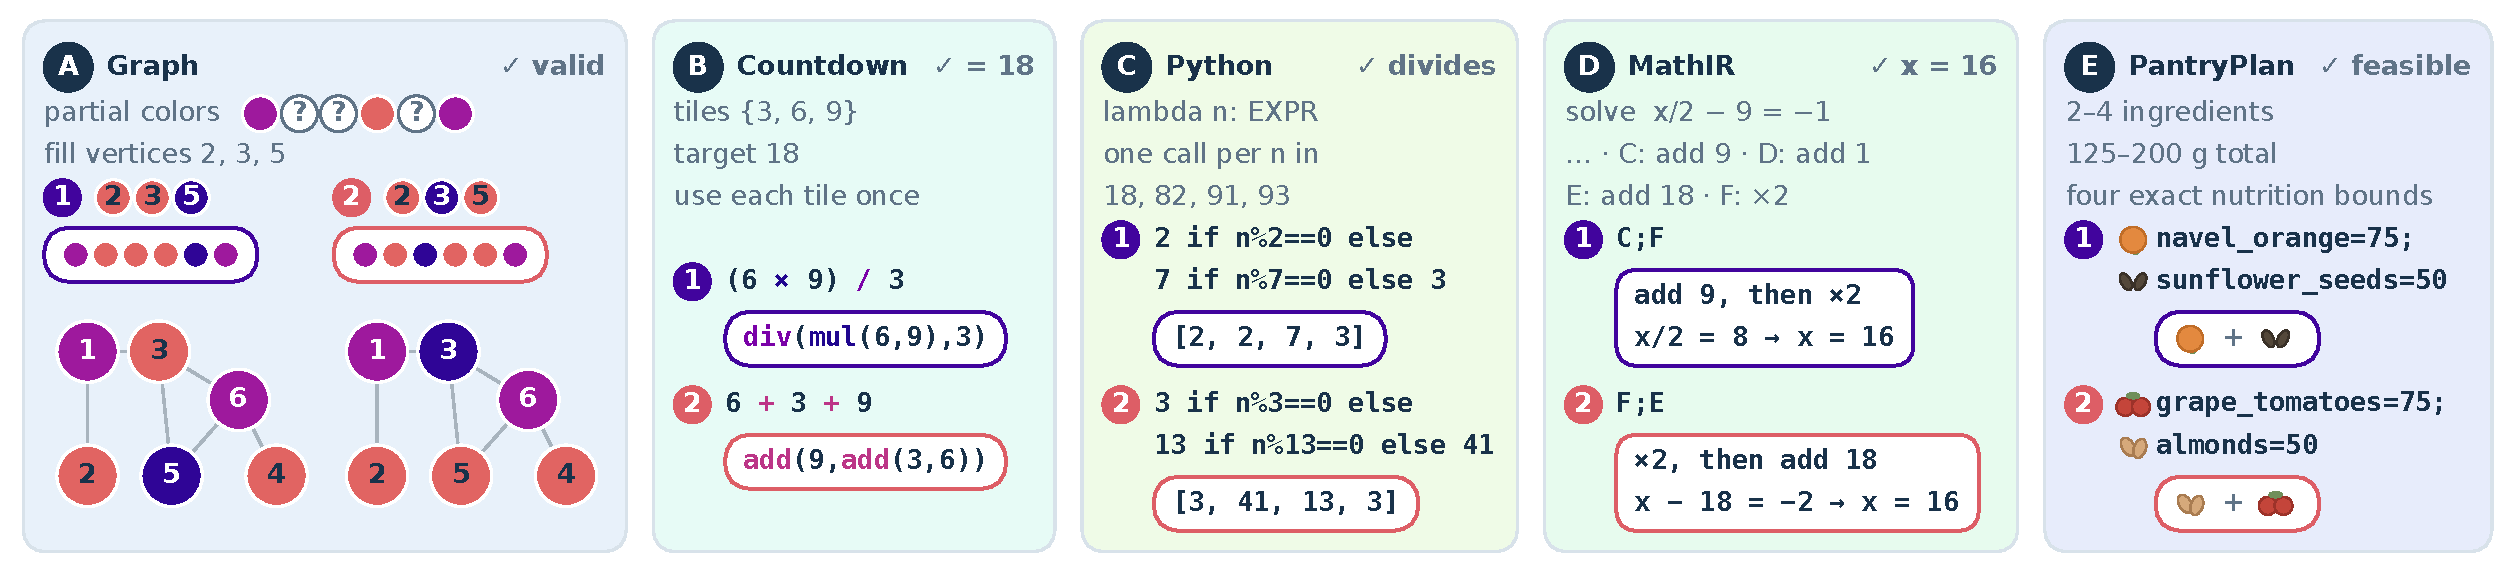
\includegraphics[width=\linewidth]{figures/modebench_examples.pdf}
  \caption{\textbf{One prompt can have different verified outputs.}
  Keys identify a color vector in Graph, a normalized computation tree in
  Countdown, an executed return vector in Python, an algebraic state trajectory
  in MathIR, or an ingredient support in PantryPlan. Cosmetic aliases merge;
  different accepted computations or configurations remain distinct under
  each domain's execution rule.}
  \label{fig:modebench-examples}
\end{figure}

Figure~\ref{fig:modebench-examples} shows the five domains. Countdown and MathIR
capture different routes to an answer, Python captures different tested
behaviors, and Graph and PantryPlan capture different valid configurations.
This distinction matters when interpreting breadth: an additional valid
configuration and an additional computation route are both verified modes,
but they are not the same kind of alternative. The keys measure executed
outputs, not latent reasoning strategies or the usefulness of a solution in
a later task. Appendix~\ref{app:domain-overview} gives the exact key and alias
rules, with verbatim prompts in Appendix~\ref{app:prompts}.

\subsection{Success and sampled breadth}
\label{sec:collapse-metrics}

For $K$ independent outputs, let $D_K$ count their distinct valid keys. Our two
primary metrics ask complementary questions:
\[
  \texttt{pass@}K=\Pr[D_K>0],\qquad
  \texttt{distinct@}K=\mathbb E[D_K].
\]
The first measures the chance of finding any correct output; the second
measures how many different correct outputs the samples contain. We use
$K=8$ throughout the training comparisons. The metrics have different units:
probability and expected verified-key count. Their numerical magnitudes
should not be compared directly, and a larger mode count can partly reflect
more successful samples rather than a more balanced correct-output distribution.

To make that coupling visible, we also report \emph{extra modes},
$\texttt{distinct@8}-\texttt{pass@8}$: the expected number of verified keys
beyond the first correct output in a sampled set. This decomposition helps
interpret a breadth gain but does not hold correctness fixed. None of these
finite-sample measurements identifies the total number of positive-probability
modes or proves that an unobserved mode has become impossible.
Appendix~\ref{app:metric-details} gives the full definitions and reference policies.

\subsection{Harder tasks with the same notion of a mode}
\label{sec:levels-design}

The benchmark has two disjoint levels for the training experiments. Level 2
adds structural difficulty while retaining each domain's validator, key,
training/evaluation sizes, and valid-mode-count histograms on those splits.
For example, Graph hides more vertices and Countdown requires more operands.
Frozen-model evaluation checks that the harder level remains solvable. This
lets us change task difficulty without changing what counts as a distinct
success; the construction and admission checks appear in
Appendix~\ref{app:data-levels}.

\section{ReplayMaxRL: Learn from New Samples and Remember Successes}
\label{sec:method}

ReplayMaxRL uses the two outputs of the validator for different purposes:
correctness rewards train on fresh samples, and canonical keys organize
memory. Both paths use policy-generated responses. The method needs neither
gold solutions nor a precomputed catalogue of valid modes.

\begin{figure}[H]
  \centering
  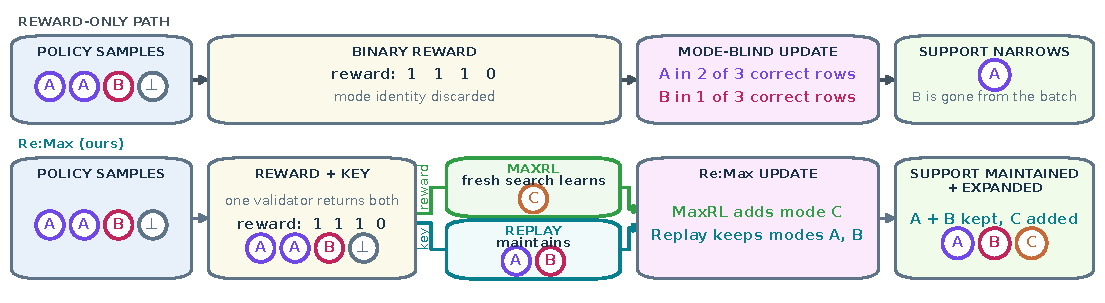
\includegraphics[width=\linewidth]{figures/verified_support_story.pdf}
  \caption{\textbf{Fresh learning and memory use the same verified samples.}
  MaxRL learns from their binary rewards. Replay stores exemplars by canonical
  key and revisits retained keys with equal weight. In the schematic, fresh
  samples add C while replay revisits A and B. A stored exemplar can continue
  to receive a training signal after it becomes rare in fresh samples.}
  \label{fig:verified-support-story}
\end{figure}

\subsection{Learning from fresh rollouts}
\label{sec:maxrl-method}

MaxRL combines success objectives across sampling budgets
\citep{tajwar2026maxrl}. With binary rewards, its centered group estimator
weights a correct response more strongly when successes in the group are
scarce. This provides a useful test of replay: memory should be evaluated
alongside an objective designed for learning from sampled successes, as well
as alongside Dr.GRPO \citep{liu2025understanding}.

Both fresh objectives still depend on what the policy currently samples.
An absent mode contributes no direct score term, and an all-correct or
all-incorrect group has zero centered task advantage. MaxRL changes the
fresh learning signal without creating a persistent record of which correct
behaviors have occurred. Appendix~\ref{app:binary-maxrl} specifies the exact
advantages and their finite-group interpretation.

\subsection{Replaying distinct verified successes}
\label{sec:replay}

Each training prompt owns an initially empty, bounded bank $\mathcal B_x$.
When a new key is admitted, the bank retains one verified exemplar $e_c$.
Repeated discoveries of that key do not add further entries. A deterministic
schedule revisits nonempty prompt banks throughout training. For an exemplar
of token length $|e_c|$, the replay loss is
\begin{equation}
 L_{\mathrm{replay}}(x)=-\frac{1}{|\mathcal B_x|}
 \sum_{c\in\mathcal B_x}\frac{\log\pi_\theta(e_c\mid x)}{|e_c|}.
 \label{eq:lm-verified-replay}
\end{equation}
Each retained key receives the same share of replay, independent of how often
it appeared in fresh rollouts. A mode discovered once therefore continues to
receive a signal alongside a mode discovered repeatedly. Token normalization
sets the loss scale for each exemplar; it does not make exemplar likelihood
equal to the total probability of generating its canonical key.

We add this loss to the fresh MaxRL update. Replacing MaxRL with Dr.GRPO yields
ReplayDr.GRPO. Replay exemplars stay outside the fresh reward group, so the
fresh objective and replay can be varied separately. The controls execute
the same bank and scoring code with zero replay gradient; their learned banks
and workloads can differ as policies diverge. Banks contain only responses to
training prompts. Held-out evaluation therefore tests what training changes
in the policy, rather than retrieving answers from the bank.
Appendix~\ref{app:algorithm} gives admission, scheduling, masking, and loss scaling.

\subsection{Why memory addresses a different pressure}
\label{sec:collapse-mechanism}

Common correct modes appear in more on-policy updates than rare correct modes,
although both receive the same binary reward. In an isolated softmax model
with independently trained logits, the mean updates of GRPO, Dr.GRPO, and
binary MaxRL amplify an initial imbalance and generically concentrate on one
correct mode. A fixed replay bank changes this flow: persistent likelihood
training supplies a qualitative probability floor for its stored modes
(Appendix~\ref{app:theory}).

Theory studies idealized mean flows. The result explains a pressure that replay
can counter; it does not certify the implemented neural optimizer. A finite
bank protects only admitted modes in the ideal analysis, and its probability
floor can be too small to yield observable samples. Our experiments therefore
measure held-out support directly and separately inspect fixed-exemplar score
trajectories. They do not infer universal preservation from the theorem.

\section{Experimental Design}
\label{sec:experiments}
\label{sec:shared-protocol}

We compare Qwen2.5-0.5B, Falcon3-1B, and Qwen2.5-3B on all five Level-1 domains.
Each run trains for eight passes with five registered seeds per comparison.
Evaluation averages four eight-sample draws on 128 held-out prompts, with
matched requests across methods. Complete paired blocks receive nominal
95\% intervals; incomplete intersections retain their exact seed counts and
are descriptive. Missing or ambiguous endpoints are not imputed. The shared
recipe and source-integrity rules are in
Appendices~\ref{app:repro-run-contract} and~\ref{app:source-integrity}.

\phantomsection\label{sec:retention-design}
The comparisons answer three questions. First, does adding canonical replay
to Dr.GRPO improve correctness and verified support across scales? Supporting
controls test reward normalization, on-policy redistribution, ordinary success
memory, and semantic exploration. UCPO and sparse RLEP-Dr are compared at
0.5B and 1B only; fixed Semantic-MaxEnt is defined in
Appendix~\ref{app:semantic-maxent}. Second, does replay still help when the
fresh objective is MaxRL?
\phantomsection\label{sec:factorial-design}
The central factorial crosses Dr.GRPO/MaxRL with replay off/on at all three
scales, yielding Dr.GRPO, ReplayDr.GRPO, MaxRL, and ReplayMaxRL.
Third, does the same pattern hold on the harder Level 2? This factorial uses
Qwen2.5-0.5B, with four complete domain comparisons and partial PantryPlan
results. Appendix Table~\ref{tab:experiment-map} gives the exact coverage.

\section{Results}
\label{sec:results}

\subsection{Experiment 1: replay improves success and sampled support}
\label{sec:results-retention}

\textbf{Replay improves success and sampled support across scales.}
Figure~\ref{fig:cross-scale-terminal-effects}A shows positive block-mean
changes in both primary endpoints for every model and domain. Raw
\texttt{distinct@8} increases in all 74 admissible seed pairs. This consistency
matters: the result spans valid configurations, computation routes, and tested
program behaviors, rather than depending on a single task or favorable seed.
The excluded Falcon Countdown run and its four-seed comparison remain
explicit in the figure and Appendix~\ref{app:source-integrity}.

\begin{figure}[!htbp]
  \centering
  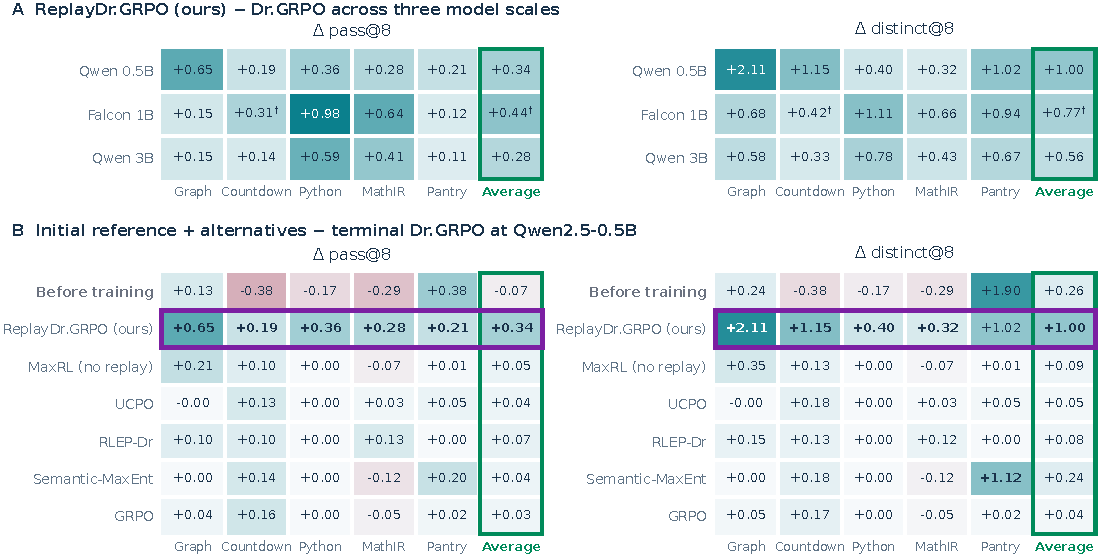
\includegraphics[width=\linewidth]{figures/experiment1_retention_comparator_matrix.pdf}
  \caption{\textbf{Canonical replay improves correctness and verified breadth.}
  (A) ReplayDr.GRPO minus Dr.GRPO at all three scales.
  (B) Qwen2.5-0.5B alternatives minus Dr.GRPO. Columns measure probability
  points and expected verified-key counts, respectively. The green Average
  weights domains equally within seed. A dagger marks four paired seeds in
  Falcon Countdown and its Average; other cells use five. Only complete
  blocks receive nominal 95\% intervals. Purple denotes ReplayDr.GRPO;
  bold entries mark column maxima in Panel B.}
  \label{fig:cross-scale-terminal-effects}
\end{figure}

Countdown provides a concrete interpretation: replay more than triples the
number of sampled verified computation routes at Qwen2.5-0.5B while also
raising correctness. Python shows why the two metrics must be read together:
its correctness improves substantially, but the gain in breadth beyond the
first correct output remains uncertain. More successful samples alone do
not demonstrate a more balanced distribution over correct outputs. The appendix reports the exact
means and uncertainty for these examples
(Appendix~\ref{app:retention-numerical-detail}).

The controls also distinguish the value of balancing keys from simply
reusing successes. At Qwen2.5-0.5B, ReplayDr.GRPO has the largest mean
correctness gain among the direct alternatives in every domain
(Figure~\ref{fig:cross-scale-terminal-effects}B). Replacing equal key weights
with weights proportional to fresh discovery frequency reduces extra modes
on average, while the aggregate correctness contrast remains inconclusive.
The advantage is concentrated in Graph, Countdown, and PantryPlan; it is not
a uniform benefit across tasks. This ablation supports key balancing as a
contributor to breadth (Appendix~\ref{app:frequency-replay-progress}).

\subsection{Experiment 2: replay complements a stronger fresh objective}
\label{sec:results-maxrl}

\textbf{Replay adds value beyond MaxRL at both scales with complete MaxRL pairs.}
The two replay comparisons in Figure~\ref{fig:maxrl-factorial} separate
memory from the choice of fresh objective. At 0.5B and 1B, replay improves
the domain-averaged correctness and raw mode count under both Dr.GRPO and
MaxRL. Thus the replay benefit persists when fresh learning already uses
MaxRL's sampling-aware objective. The comparison identifies the effect of
adding the replay update; it does not establish which individual stored modes
account for the held-out gains.

\begin{figure}[!htbp]
  \centering
  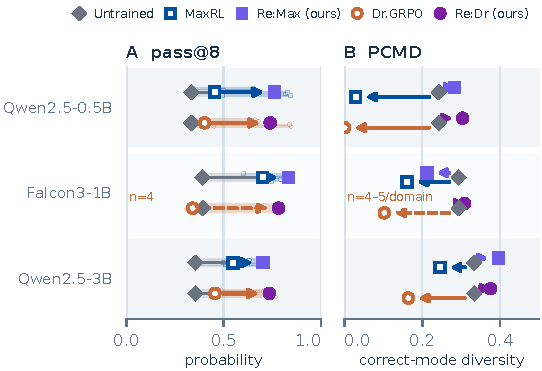
\includegraphics[width=\linewidth]{figures/e118_all_scale_factorial_progress.pdf}
  \caption{\textbf{Replay complements both fresh objectives at multiple scales.}
  Each row shows Dr.GRPO/ReplayDr.GRPO and MaxRL/ReplayMaxRL on both endpoints.
  Diamonds are initial models; open/filled markers are training without/with
  replay. Complete tracks average domains within seed; faint paths show seeds.
  Falcon Dr.GRPO uses four common seeds. The dashed 3B MaxRL track averages
  domain-specific paired means equally ($n=5,3,5,3,1$ for
  Graph/Countdown/Python/MathIR/Pantry), with no common-seed trajectory or interval. Appendix
  Figure~\ref{fig:maxrl-factorial-scale-extensions} reports each domain's
  correctness and verified-mode results at every scale.}
  \label{fig:maxrl-factorial}
\end{figure}

The effect is not identical across domains or scales. ReplayMaxRL improves
both endpoints in every 0.5B domain. At 1B, mean correctness improves in every
domain, but Graph's mean raw-support effect is negative and inconclusive.
The 3B Dr.GRPO comparison is complete. For 3B MaxRL, Graph and Python are
complete while the other domains have smaller paired cohorts. The descriptive
3B average also favors ReplayMaxRL on both endpoints. We retain all three
model rows in the main figure, while distinguishing this partial summary
from the complete scale comparisons.
Appendix~\ref{app:factorial-numerical-detail} gives the aggregate estimates;
Appendix~\ref{app:factorial-training-curves} shows both metrics throughout training.

\subsection{Experiment 3: replay on harder matched tasks}
\label{sec:results-levels}

\textbf{Replay improves both average endpoints at both difficulty levels.}
Figure~\ref{fig:level2-admission} compares the four domains with complete
factorials at Qwen2.5-0.5B. Their aggregate moves toward greater correctness
and sampled support with replay under either fresh objective, at both levels.
The levels preserve the mode definition and the distribution of valid-mode
counts while changing task structure, so the comparison tests more than a different key
definition. PantryPlan remains outside this aggregate because its Level-2
factorial is incomplete.

\begin{figure}[!htbp]
  \centering
  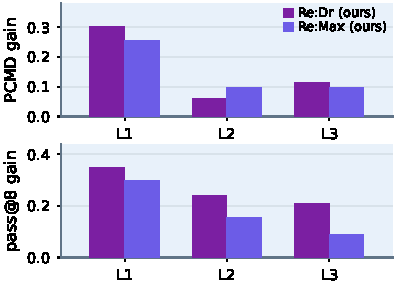
\includegraphics[width=.98\linewidth]{figures/modebench_level_admission.pdf}
  \caption{\textbf{Replay across difficulty levels at Qwen2.5-0.5B.}
  Open/filled markers denote Level 1/2. (A) Frozen-model success in all five
  domains. (B) Terminal means over Graph, Countdown, Python, and MathIR,
  weighted equally within each of five paired seeds. Both levels and all four
  methods share this completed cohort. Partial PantryPlan arm counts are
  reported separately (Appendix~\ref{app:level2-interim}).}
  \label{fig:level2-admission}
\end{figure}

Graph supplies the clearest domain-level evidence: both replay variants
improve correctness and raw support substantially on the harder problem.
The other completed domains' correctness and raw-support intervals include
zero. We therefore interpret the aggregate as evidence that replay can remain
useful under this controlled increase in difficulty, not as a universal gain
on harder tasks. Appendix~\ref{app:levels-numerical-detail} reports the Graph
estimates, and Appendix~\ref{app:level2-interim} gives all fresh-objective
and replay-interaction contrasts.

\section{Related Work}
\label{sec:related}

Prior work documents reduced output diversity under RLHF and reasoning RL,
declining entropy, and reduced high-budget problem coverage
\citep{kirk2024understanding,dang2025diversity,cui2025entropy,yue2025rlvrlimit}.
\mb{} instead measures different verified outcomes within one prompt.
Semantic clustering infers equivalence from language
\citep{farquhar2024detecting}; our keys come from accepting execution.
Sampling-based selection makes the proposal distribution relevant to reasoning
\citep{brown2024monkeys,snell2024testtime,cobbe2021training,lightman2023lets},
but our experiments do not measure the downstream value of each alternative.

Outcome bonuses, set objectives, distribution matching, and uniform-correct
objectives encourage broader support
\citep{song2025outcome,chen2025passktraining,li2025divergence,
li2026setpo,li2026distribution,lochab2026ucpo}. MaxRL combines objectives across
sampling budgets \citep{tajwar2026maxrl}; we test whether explicit memory adds
to it. Replay reuses experience and can mitigate forgetting
\citep{lin1992selfimproving,rolnick2019replay}, including successful reasoning
trajectories in RLEP \citep{zhang2025rlep}. Our bank groups successes by
execution key and balances those keys independently of discovery frequency,
connecting success replay with behavioral archives in quality-diversity methods
\citep{mouret2015illuminating,ecoffet2021return}.

\section{Conclusion}
\label{sec:conclusion}
\label{sec:discussion}
\label{sec:limitations}

Learning to produce a correct answer and keeping different correct answers
available are separate properties of training. \mb{} makes the second
property measurable through executable output identities. ReplayMaxRL uses
those same identities as memory: fresh learning improves the policy from new
samples, while replay keeps stored successes involved in training. The matched
comparisons show that this can improve held-out correctness and sampled
verified breadth, including beyond MaxRL.

\phantomsection\label{sec:hosted-concentration}
The measurement also applies beyond these training runs. Inference-only tests
of GPT-5.6 Sol and Claude Opus 5 find highly accurate yet concentrated Graph
outputs (Appendix~\ref{app:hosted-comparison}). These observations illustrate
the distinction between correctness and breadth; they identify neither a
training cause nor a model-size effect.

Our claims concern sampled, task-defined outputs. Replay cannot retain a mode
before discovering and storing it, and improved held-out breadth does not
show that every stored exemplar survives. A fixed-bank audit finds improving
central scores alongside a declining tail
(Appendix~\ref{app:fixed-bank-survival}); exact mode probabilities remain
unverified. The idealized theory does not certify neural training, and the
experiments do not show that breadth causes the accuracy gains. The next
question is whether retaining verified alternatives helps an agent recover
from a failed approach or adapt when constraints change. The benchmark and
method provide a controlled way to begin testing that question.
\label{sec:main-end}

\clearpage
\phantomsection\label{sec:references}
\bibliographystyle{iclr2027_conference}
\bibliography{example_paper}

